\documentclass[a4paper]{article}

%% Useful packages
\usepackage{amsmath}
\usepackage{graphicx}	
\usepackage{algpseudocode}
\usepackage{algorithm}
\usepackage[colorinlistoftodos]{todonotes}
\usepackage[colorlinks=true, allcolors=black]{hyperref}
\usepackage[fontsize=11pt]{scrextend}
\usepackage{titlesec}
 \usepackage[section]{placeins}

\setlength\parindent{0pt}
\titleformat*{\section}{\Large\bfseries}
\titleformat*{\subsection}{\Large\bfseries}

\title{PowerEnjoy Service - Integration Test Plan Document}

\begin{document}

\begin{titlepage}
\begin{figure}
\centering

\includegraphics[width=0.2\textwidth]{polimi.jpg}
\par
\LARGE Politecnico di Milano
\end{figure}


\maketitle
\textbf{Version 1.1}
\newline

\raggedright
Authors:
\begin{itemize}
	\item Domenico FAVARO (Mat. 837995)
        	\item Matheus FIM (Mat. 876069)
	\item Caio ZULIANI (Mat. 877266)	
\end{itemize}
\raggedleft
Prof. Elisabetta DI NITTO
\thispagestyle{empty}
\end{titlepage}

\tableofcontents
\newpage
 
\section{Introduction}
\subsection{Revision History}
This section records all revisions to the Document.
\newline \newline
\begin{tabular}{ | c | c | c | c | }
\hline
	Version & Date & Authors & Summary \\ \hline
	1.1 & 15/01/16 & Domenico Favaro, Caio Zuliani, Matheus Fim & Initial Release  \\ \hline
\end{tabular}

\subsection{Purpose and Scope}
The Integration Test Plan Document (ITPD) serves to present the integration sequence and testing for all Subsystems and Components that conform PowerEnjoy Car Sharing Service. This is a key part to guarantee the functioning and quality of the software. The Document will present the division of the System in Subsystems and Components that will endure individual testing as independent modules and then be subject to integration on the whole System.

\subsection{Definitions and Abbreviations}
\begin{itemize}
\item \textbf{RASD:} Reqirements And Specifications Document.
\item \textbf{DD:} Design Document.
\item \textbf{ITPD:} Integration Test Plan Document.
\item \textbf{SDK:} Software Development Kit
\item \textbf{App:} Application, refering to Web or Mobile App.
\item \textbf{Subsystem:} Part of the system the generally encapsulates one or more features.
\item \textbf{Component:} Self sustained part of the System that provides with functionalities and is part of one or more subsystems.
\item \textbf{Bottom-up:} Referring to Bottom-up testing. Each component at lower hierarchy is tested individually and then the components that rely upon these components are tested.
\item \textbf{Top-down:} Top-down integration testing is an integration testing technique used in order to mock or simulate the behaviour of the lower-level modules that are not yet integrated.
\item \textbf{Mock:}Simulation that mimic the behavior of certain objects and fucntions in controlled ways, done to test the behavior of some other object.
\end{itemize}
For other concepts concerning the Service definition look in the \textbf{Glossary} section of the RASD and DD.

\subsection{Reference Documents}
\begin{itemize}
\item Specification Document: Assignments AA 2016-2017.pdf
\item PowerEnjoy Requirements And Specifications Document (RASD)
\item PowerEnjoy Design Document (DD)
\item Example Document - Integration testing example document.pdf
\item Testing Tools Documents:
\begin{itemize}
\item[-] Mockito
\item[-] JMeter
\end{itemize}
\end{itemize}

\newpage
\section{Integration Strategy}
\subsection{Entry Criteria}
We define the criteria that must be met before integration testing of the system components. We consider Integration a part of the production development. In order for production to start all documentation must first be written and up to date, including RASD and DD, to have a clear and full scope of the system components functionalities and importance. Once in production, the integration of a singe component can be done when the following criteria is met:
\begin{itemize}
\item The Component feature must be 100\% complete, that is all classes and functions must have been implemented.
\item No tickets must be opened for the Component, no bugs or cosidered missing features must be present.
\item Individual component testing must have been performed, using JUnit to test its classes and functions.
\item All the interfaces the Component has to communicate to have to be present or at least mocked to be able to test its coupling.
\end{itemize}
  
\subsection{Elements to be Integrated}
As stated in the Design Document, our system is composed by several High level Components presented in 3 tiers. Specifically these components are:
\begin{itemize}
\item Client Tier:
\begin{itemize}
\item[-] User Client Component
\item[-] CRM Client Component
\item[-] Car Component
\end{itemize}
\item Server Tier:
\begin{itemize}
\item[-] User Controller
\item[-] CRM Controller
\item[-] Car Controller
\item[-] Reservation Controller
\item[-] Ride Controller
\item[-] Payment Controller
\item[-] User Report Controller
\item[-] Email Helper
\item[-] Location Helper
\item[-] Chat Service
\end{itemize}
\item EIS Tier:
\begin{itemize}
\item[-] Database
\end{itemize}
\end{itemize}

\subsection{Integration Testing Strategy}
Our approach following the 3-tiered structure will follow a \textbf{Bottom-up} strategy, working on components that do not depend on others to function first. \par
This implies following the next tier order: EIS -\(>\) Server -\(>\) Client for development and testing.\par
Inside each Tier Bottom-up strategy will be used again to integrate independent modules first and then those that depend on others.This strategy will help in contrast to Top-down to minimize the mock-up testing to be done, testing on top of already deployed modules. The order in which the 'Bottom' modules will be picked will follow a Critical-Module-First Integration Strategy, giving priority to those that will have dependencies of other modules, this will help not only to spot any error on critical modules first but also to unblock the integration of dependant modules earlier on.

\subsection{Sequence of Component/Function Integration}
Following the Bottom-up strategy we'll integrate the components that have no dependencies on other modules. First we'll present the component integration within each subsystem and then the subsystems integration order.
\subsubsection{Software Integration Sequence}
For each subsystem, we'll identify the sequence in which the software components will be integrated within the subsystem.
\paragraph{EIS Tier - DBMS:}
As shown in the DD our DBMS is not dependent on any module and even if it's a System already present for some structures (Cars, CRM) we have to add the entities that we'll serve the purpose of our System, that is Users, Reservations, Rides, Payments, User Reports. These will be entities that will be added by our System, specifically be the Controllers so this module has to be integrated first to answer the queries for the rest of the subsystems.
\paragraph{Server Tier:}
In the DD we present the High level Component structure. Based on the dependencies shown in this structure we'll select the order to test and deploy these components.
\begin{figure}[h]
\centering
\vspace*{\fill}
\noindent\makebox[\textwidth]{\includegraphics[width=1.4\textwidth]{HighLevelComponents.png}}%
\caption {Component Structure}
\vspace*{0.5cm}
\end{figure}
The Helper Components depend on no other components so according to the Bottom-up strategy they will be the first ones to integration. However not all Helpers are critical to other components so we'll prioritize the Critical Helper Components first, that is Location Helper as User, Car and Ride Controllers depend on it.\par
For each controller we have to implement Entity and Session Beans that will contain the methods and functions for managing the corresponding entites and logic so everyone of them will have Data Access Utilities to communicate with the DBMS. Their Integration order will then depend on the other controllers they depend on, meaning the other controllers they have to interface with.\par
\newpage
An arrow suggest the Component on the right depends on the one on the left and will be integrated after all the previous one have been integrated.
\begin{figure}[h]
\centering
\vspace*{\fill}
\noindent\makebox[\textwidth]{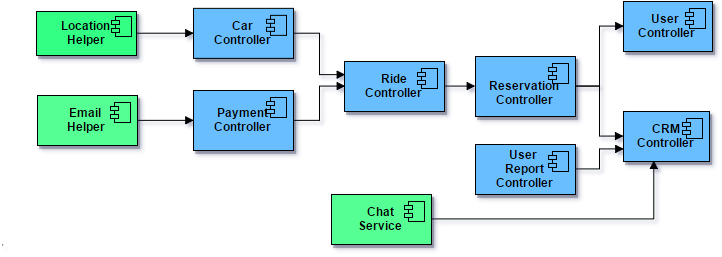
\includegraphics[width=1.4\textwidth]{ServerIntegrationSequence.png}}%
\caption {Server Components Integration}
\vspace*{0.5cm}
\end{figure} 

\paragraph{Client Tier:}
The Client Tier is based in two main components, User and CRM. Even if they are different they share many common functionalities including Login, Car Localization, Car Detail and Chat Service. They can be deployed simultaneously as they do not depend on each other and to test the logic subsystem from the Client side we can deploy one functionality at a time when all the dependencies have been met.

\newpage
\begin{figure}[h]
\centering
\vspace*{\fill}
\noindent\makebox[\textwidth]{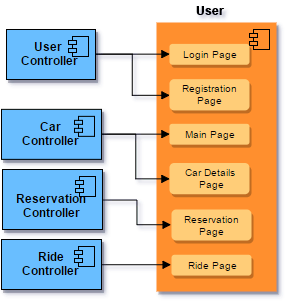
\includegraphics[width=0.45\textwidth]{UserComponentDependencies.png}}%
\caption {User Component Dependencies}
\vspace*{0.5cm}
\end{figure} 

\begin{figure}[h]
\centering
\vspace*{\fill}
\noindent\makebox[\textwidth]{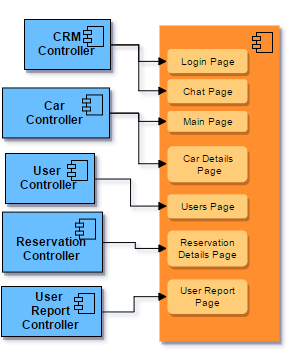
\includegraphics[width=0.45\textwidth]{CRMComponentDependencies.png}}%
\caption {CRM Component Dependencies}
\vspace*{0.5cm}
\end{figure}
 
\newpage
\subsubsection{Subsystem Integration Sequence}
As mentioned before our subsystems corresponging to the Data, Logic and Presentation Tier will be integrated in that order. Before integrating a subsystem all the components inside it must be integrated as well.
\begin{figure}[h]
\centering
\vspace*{\fill}
\noindent\makebox[\textwidth]{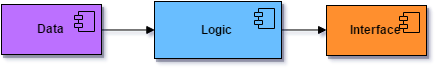
\includegraphics[width=0.9\textwidth]{SubsystemsDependencies.png}}%
\caption {Subsystem Integration Sequence}
\vspace*{0.5cm}
\end{figure}


\newpage
\section{Individual Steps and Test Description}
\newpage

\section{Performance Analysis}

Even tough the performance analysis is evaluated within the system as a whole, it was agreed that while testing the components, the isolated performance will be taken into account, as to correct unacceptable behavior, such as too slow response time, as soon as possible. 

The aim of the performance analysis is to check the reliability of the application under normal usage conditions, providing benchmarks and identifying the response time, utilization and throughput of the application. So, for this test, the expected workload should be considered as in terms of the biggest city where the application will be implemented, taking into account an average usage for a long period with peaks of heavy traffic. 

Also, For this part of the testing it is needed to consider the performance of all the different interfaces of the system. Particularly, the mobile application, the web application and the screen inside the car should all have satisfactory behavior, considering all kinds of users that can operate each interface. 

Some important requirements to be evaluated:
\begin{itemize}
\item[-] For the mobile application it is considered that the target public of the app can have any kind of Smartphone. So, the test will be made in low-end devices. This includes low ram availability, small internal space allocation and low processing power capacity.
\item[-] All the interfaces need to respond properly with slow network situations, and be reliable in situations of unstable network. 
\end{itemize}
\newpage


\section{Required Tools and Test Equipment}
\subsection{Tools}
\subsection{Test Equipment}

\section{Required Program Stubs and Test Data}
\subsection{Program Stubs}
\subsection{Test Data}

\newpage
\section{Effort Spent}
\begin{tabular}{ | c | c | c | c | }
\hline
	\textbf {Date} & \textbf {Domenico} & \textbf {Caio} & \textbf {Matheus} \\ \hline
	27/12/16& 2h & 2h & 2h  \\ \hline
	28/12/16& - & - & - \\ \hline
	29/12/16& 1h & - & - \\ \hline
	30/12/16& 2h & - & - \\ \hline
	31/12/16& - & - & - \\ \hline
	01/01/17& - & - & - \\ \hline
	02/01/17& 2h & - & - \\ \hline
	03/01/17& 2h & - & - \\ \hline
	04/01/17& 2h & - & - \\ \hline
	05/01/17& - & - & - \\ \hline
	06/01/17& - & - & - \\ \hline
	07/01/17& - & - & - \\ \hline
	08/01/17& - & - & 6h \\ \hline
	09/01/17& - & - & - \\ \hline
	10/01/17& - & - & - \\ \hline
	11/01/17& - & - & - \\ \hline
	12/01/17& - & - & - \\ \hline
	13/01/17& - & - & - \\ \hline
	14/01/17& - & - & - \\ \hline
\end{tabular}
\newpage

\section{Changelog}
As the project and design decisions may change during the development this document is also prone to change.
We'll document every version in this part.
\begin{itemize}
\item \textbf {Version 1.1:} 15/01/2017
\end{itemize}
\end{document}
